\section{Research Topic Summary}

Use sections to organize your contents. Read the project proposal guidelines available on Moodle to get more information on the contents your proposal should cover. Do not forget to cite online sources~\cite{WFR2017}, books~\cite{grus2019data} or articles you are referencing! It may also be useful to integrate charts or figures in your proposal as seen in Figure~\ref{fig:example}.

\begin{figure}[h]
  \centering
  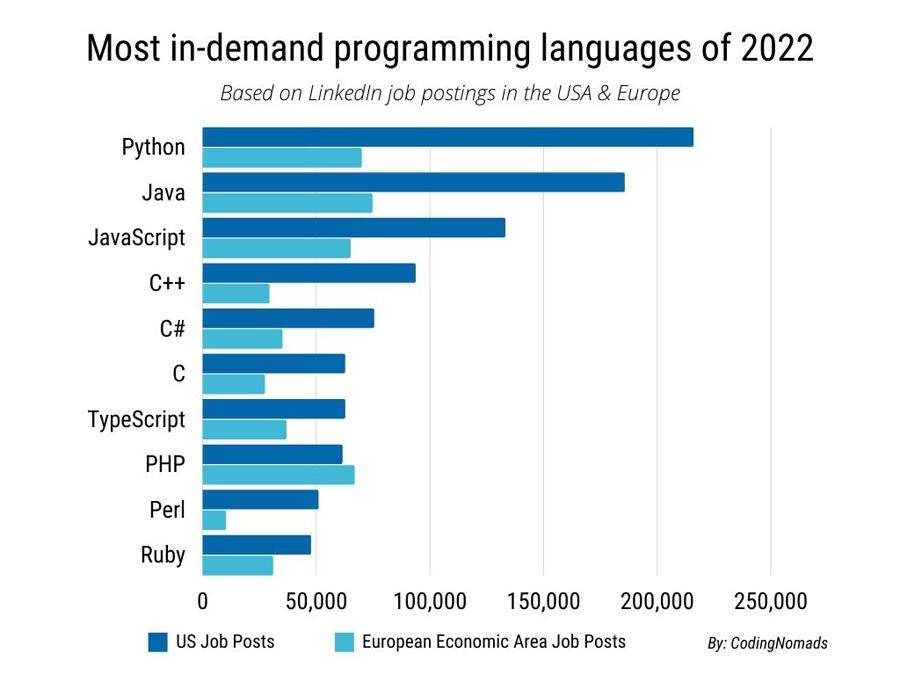
\includegraphics[scale=0.3]{figures/most-in-demand-programming-languages-of-2022-codingnomads.jpg}
  \caption[]{An example chart showing the change of popularity of
    various programming languages, taken from techrepublic Website\footnotemark[1].}
  \label{fig:example}
\end{figure}

\footnotetext[1]{\url{https://www.techrepublic.com/article/the-best-programming-languages-to-learn-in-2022/}}

In the Latex source provided together with this PDF, you also find hints on how to work on one Latex project collaboratively.